\section{Classification Methodology}
\label{sec:classification-methodology}

\platname offers a network perspective of the mobile Internet traffic.
To detail the mobile traffic, we need to first identify the access technology used by the devices, and the applications and Web-services responsible for each flow captured by \platname.
In this section we describe the technique we used to identify the access technology and the applications and Web-services. 

\subsection{Access Technology Classification}

To quantify the impact of the access technology, we need to first identify the access technology used by the devices when accessing the Internet via \platname servers.
A mobile devices can access the Internet using either \wifi or cellular networks. 
We estimate the access technology with the description of the AS through which the mobile client connects to our \platname server. 
We get this AS description by performing a \emph{WHOIS} lookup on the IP address used by the mobile client to tunnel Internet traffic. 
For our analysis, we use the WHOIS databases available at \emph{whois.cmyru.com} and \emph{utrace.de}.
We use the information from these \emph{WHOIS} databases to manually classify the ASes to be either cellular or \wifi.
Our dataset consists of data traffic from 54 distinct ASes, of which we classify 9 to belong to cellular networks.
Each device connected our \platname server from at most two distinct ASes during the measurement study.
In contrast, a median of 4 \wifi ASes were observed per device and for one device we observed traffic from 25 different \wifi ASes that were spread across 5 countries. 

\subsection{Classification of Mobile Services}

The data traffic from mobile devices is because of the applications running on the device and OS services and libraries used by the applications. 
To analyze the behavior of mobile services we need to first associate the observed flows with the applications and the OS services responsible for the flows.
For our analysis, we focus on identifying the OS services and the applications and Web-services responsible for HTTP and SSL flows, the largest sources of mobile Internet traffic~\cite{maier:mobtraffic,falaki:mobileusage,xu:appusage}.

%The HTTP headers for HTTP Request, HTTP Response, and HTTP Entity contain a wealth of information including \useragent, \httphost, \emph{Referrer}, \emph{Content-Type}, and \emph{Content-Encoding} that can be used to classify HTTP traffic~\cite{rfc:http}.
%We now discuss the usefulness of the \useragent field to identify iOS applications show how other fields such as \httphost are essential to identify Android applications. 
%Similarly, for the SSL traffic we show that a combination of \sslservername and the DNS queries can be used to classify SSL traffic. 

\begin{table}
\begin{small}
\begin{center}
\begin{tabular}{|p{0.15\columnwidth}|p{0.12\columnwidth}|r|r|r|r|}
\hline
\multirow{2}{*}{\bf IP Protocol} & \multirow{2}{*}{\bf Service} & \multicolumn{2}{|c|}{\bf Android} & \multicolumn{2}{|c|}{\bf iOS} \tabularnewline
\cline{3-6}
           &           &  \textbf{Cell.}  &  \textbf{\wifi}  &  \textbf{Cell.}  &  \textbf{\wifi}  \tabularnewline
\hline
\multirow{3}{*}{TCP}
       &  HTTP  & 35.386 & 68.686 & 52.109 & 75.506 \tabularnewline
\cline{2-6}
       &  SSL   & 61.135 & 27.366 & 46.765 & 18.777 \tabularnewline
\cline{2-6}
       &  other & 2.346  & 3.290  & 0.256  & 1.818 \tabularnewline
\hline
\multirow{2}{*}{UDP}
       &  DNS   & 0.682  & 0.496  & 0.545  & 0.305  \tabularnewline
\cline{2-6}
       &  other & 0.316  & 0.098  & 0.286  & 3.583  \tabularnewline
\hline
 Other &  -     & 0.135  & 0.064 & 0.039  & 0.011  \tabularnewline
\hline
\multicolumn{2}{|c|}{\emph{total}} & 100.00 & 100.00 & 100.00 & 100.00 \tabularnewline
\hline
\end{tabular}
\end{center}
\end{small}
\caption{Traffic volume (in percentage) of popular protocols and services on Android and iOS devices over cellular and \wifi.
\emph{TCP flows are responsible for more than 90\% of traffic volume. Traffic share of SSL over cellular networks is more than twice the traffic share of SSL over \wifi.}} 
\label{tab:summaryIOSAndroidTraffic}
\end{table}

We begin our identification process using the classification provided Bro~\cite{bro}.
Bro uses the protocol field in the IP header to broadly classify the flows, and we use this classification to label flows as either TCP, UDP, or \emph{other}.
Bro further classifies TCP flows using well defined port numbers, and we use this classification to label flows as either HTTP, SSL (which includes HTTPS, IMAP, etc.) or \emph{other} flows.
Similarly, we use Bro to label UDP flows as either DNS or \emph{other}. 
Indeed, in \fref{tab:summaryIOSAndroidTraffic}, we observe that more than 92\% of the traffic in our \mobWild dataset is either HTTP or SSL. 
We also observe that the share of HTTP volume over \wifi and cellular are significantly different. 
This increase is a result of the reduced share of media traffic and the use of email and for social networking applications that rely on SSL.
%We detail the HTTP and SSL traffic from iOS and Android devices in \fref{sec:}

\subsubsection{HTTP Traffic Classification}

Web-services rely on the \useragent field to distinguish HTTP flows from their mobile applications from the flows originating from Web-browsers.
In our controlled experiments we observed a valid \useragent string in more than 99\% of the HTTP flows from Android and iOS.
However, because the mobile applications use built in OS services and libraries to download media content, we do not observe the identifier of the application using the OS service and library in the \useragent string for media traffic. 
For example, when an iOS devices is used to stream YouTube video on a YouTube Application or if the video is viewed on clicking a video link on Facebook application, we observe that the media content is downloaded by AppleCoreMedia service of iOS~\cite{apple:coremedia}. 
We now show how a combination of \useragent and \httphost can be used to identify either the Web-service or the application associated with the flow.

\begin{figure}
\subfloat[iOS]{\label{fig:http-wordcloud-ios}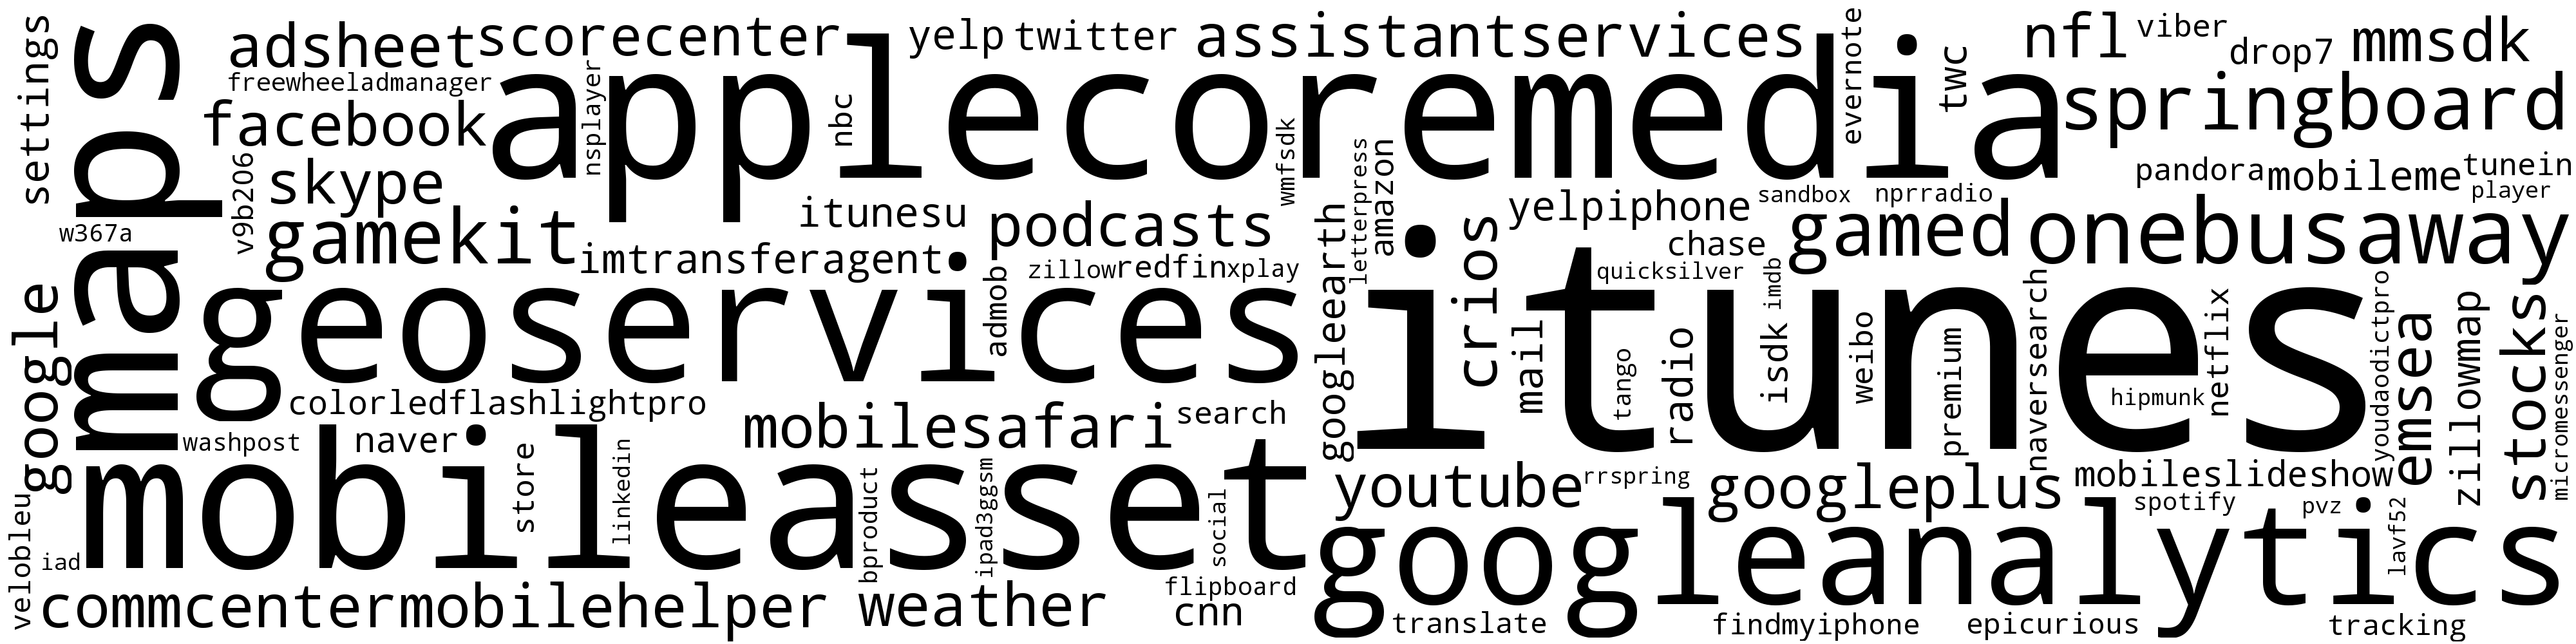
\includegraphics[width=\columnwidth]{figures/wordcloud_useragentsignature_ios_image.png}}\newline
\subfloat[Android]{\label{fig:http-wordcloud-android}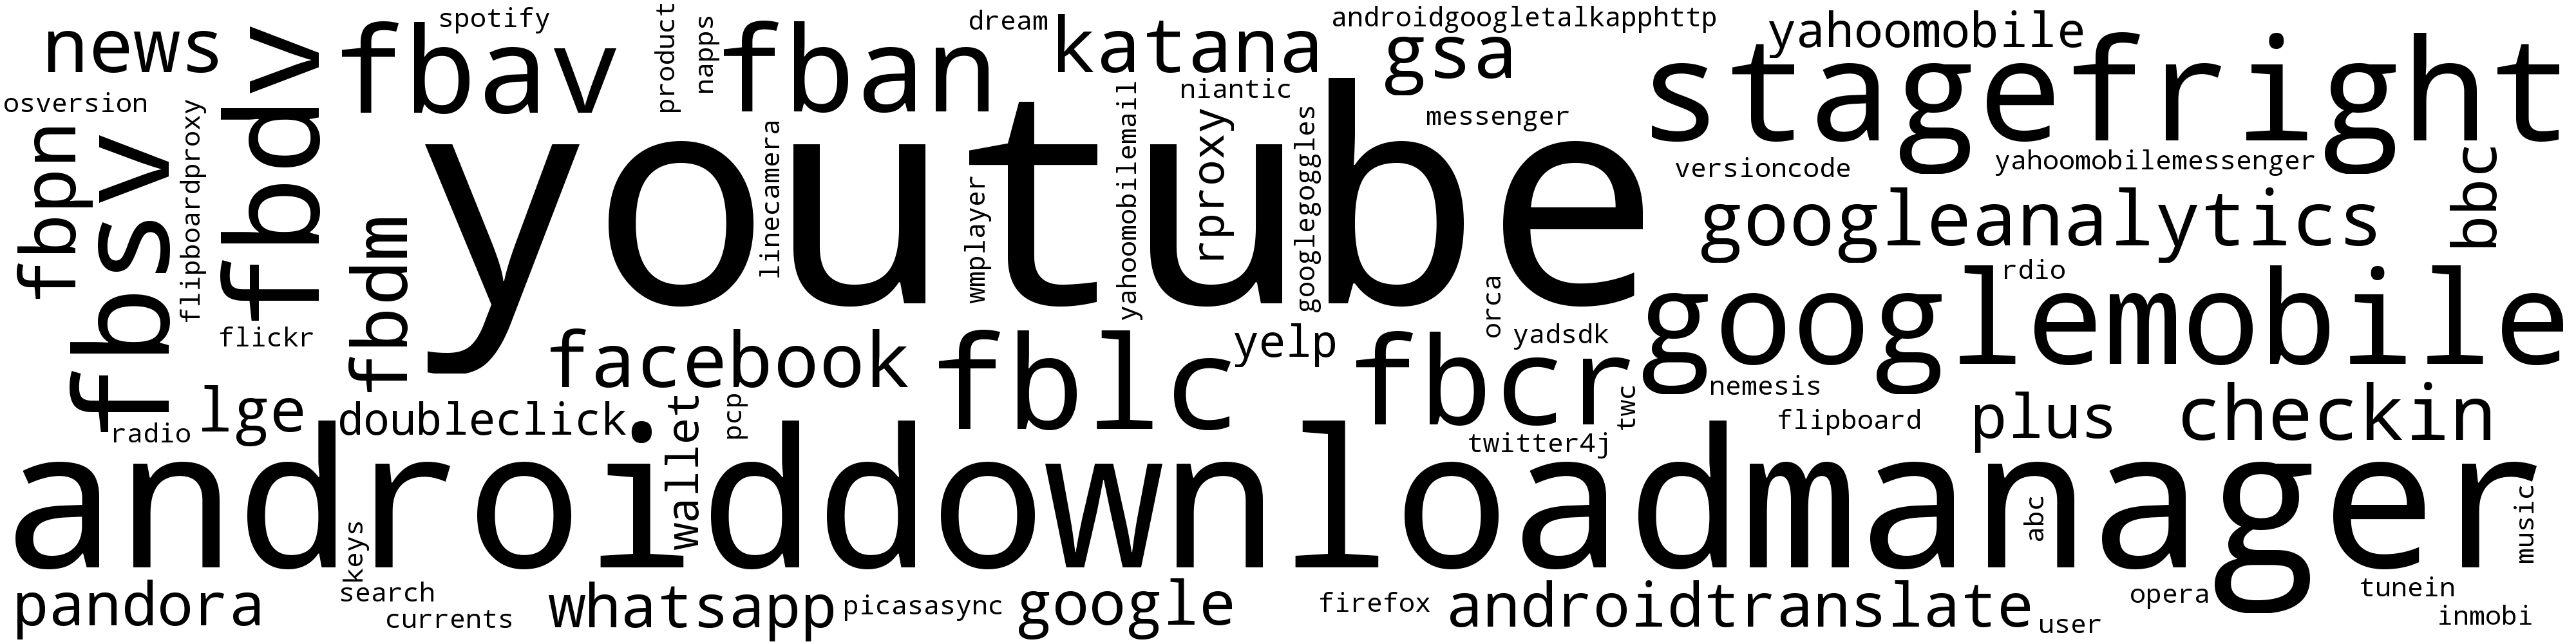
\includegraphics[width=\columnwidth]{figures/wordcloud_useragentsignature_android_image.png}}
\caption{\useragent signatures in  iOS and Android HTTP flows. \emph{The font weight represents the number of users for which a particular signature was observed.}}
\label{fig:http-wordcloud}
\end{figure}

We observe that more than 98\% of HTTP traffic from Android and iOS devices in the \mobWild dataset have a valid \useragent string; we observe a total of 1435 unique \useragent strings across Android and iOS devices. 
These \useragent strings contain an application identifier and other auxiliary information such as details of the OS, manufacturer, display resolutions, carrier, and information such as versions and compatibility with other browser engines~\cite{mozilla:useragentdetection}. 
We use regular expression to extract the tokens that contain the application information, and cluster these tokens using edit distance\footnote{We plan to release this code along with \platname package.}.
At the end of this process we were able to identify 361 unique signatures which we resolve as either applications or OS services. 

In \fref{fig:http-wordcloud} we present a \emph{word cloud} of the signatures we were able to extract from \useragent field; the text size of the signature represents the number of users for which the signature was observed.
Despite the usefulness of the \useragent, we observe that relying only on the \useragent is not sufficient to identify the application.
For example, we observe the signatures \emph{applecoremedia} and \emph{stagefright} in the \emph{word cloud} for iOS devices and Android devices, signatures of the OS services responsible to download media content.

The iOS devices rely on AppleCoreMedia service~\cite{apple:coremedia} to download media content.
We therefore observed the signature of AppleCoreMedia in more than 98.45\% of the content downloaded from the YouTube servers (which we identify based on the \httphost field in the \httpget requests). 
Similarly, depending the Android version we observe either the signature for Stagefright\cite{android:stagefright} or no application or OS service signature for YouTube traffic to Android devices. 
Indeed, we observed signatures for popular media services such as Netflix, YouTube, Vimeo, Pandora, etc. in the \httphost field in the majority traffic from iOS devices and Android devices. 
We therefore used the \httphost field to classify media content.

\begin{table}
\centering
\begin{small}
\begin{tabular}{|p{0.25\columnwidth}|c|c|c|c|}
\hline
\multirow{2}{*}{\bf Category} & \multicolumn{2}{c|}{\bf iOS} &  \multicolumn{2}{c|}{\bf Android} \tabularnewline
\cline{2-5}
  & {\bf Bytes}  & {\bf Flows} & {\bf Bytes} & {\bf Flows}   \tabularnewline
\hline
Media (Popular)         & 51.405  & 12.131 & 65.922 & 22.377 \tabularnewline
\hline
Application             & 33.987  & 80.758 & 31.353 & 77.498 \tabularnewline
\hline
Media (Ambiguous)       & 14.572  &  5.914 &  2.712 &  0.044 \tabularnewline
\hline
Other                   &  0.036  & 1.1963 &  0.013 &  0.081 \tabularnewline
\hline
{\em total}            & 100 & 100 & 100 & 100 \tabularnewline
\hline
\end{tabular}
\end{small}
\caption{Classification of HTTP Traffic.}
\label{tab:classify-http}
\end{table}

In summary, we use a combination of \useragent and \httphost field in HTTP headers to classify HTTP traffic.
In \fref{tab:classify-http}, a table that provides an overview of our classification results.
We observe that we were able to classify more than 98\% of the traffic in terms of flows and bytes from iOS and Android devices using the \useragent and the \httphost field. 
We observe that media from popular hosts contribute to more than 50\% of the traffic volume from iOS and Android devices.
Similarly, we were able to identify applications for more than 77\% of flows from Android and iOS devices. 
However, we observe media (identified based on the \useragent) served from CDNs and others hosts from which we could not identify the webservice from other fields in the HTTP header and the DNS responses before the HTTP flows to be 14.5\% of the traffic volume for the iOS devices in our dataset.

\subsubsection{Classification of SSL Traffic.}

Unlike HTTP flows, SSL flows provide limited information that can be used to identify the applications. 
Because the SSL flows do not provide any hints that point to the application, our objective of SSL classification was to identify the Web-services that are responsible for the flows. 
We now show how we used the port number, subject field in the certificate, and DNS queries to classify SSL traffic. 
Services such as mail, instant messaging, and notifications are documented to use dedicated port numbers of their traffic. 

\begin{table}
\centering
\begin{small}
\begin{tabular}{|p{0.25\columnwidth}|c|c|c|c|}
\hline
\multirow{2}{*}{\bf Service} & \multicolumn{2}{c|}{\bf iOS} &  \multicolumn{2}{c|}{\bf Android} \tabularnewline
\cline{2-5}
  & {\bf Bytes}  & {\bf Flows} & {\bf Bytes} & {\bf Flows} \tabularnewline
\hline
HTTPS                   & 91.287 & 81.960 & 97.852 & 97.168    \tabularnewline
\hline
Mail                    &  6.700 & 15.872 & 0.689  & 0.320  \tabularnewline
\hline
Notification            &  1.412 & 1.553  & 1.321  & 2.100  \tabularnewline
\hline
Other                   &  0.601 & 0.615  & 0.138  & 0.412 \tabularnewline
\hline
{\em total}             & 100 & 100 & 100 & 100 \tabularnewline
\hline
\end{tabular}
\end{small}
\caption{Classification of SSL Traffic based on port number. \emph{HTTPs is the most popular service that uses SSL in the \mobWild dataset.}}
\label{tab:classify-ssl-port}
\end{table}

SSL is used by mobile devices for various services including mail, notifications, instant messaging, and web browsing.
On using the port number of classify SSL traffic,  we observe in \fref{tab:classify-ssl-port} that a majority of SSL traffic by volume and flows is HTTPS.
The rest of the traffic is either Mail, Notification services, or other services such as instant messaging.

We first use the common name (CN) field of certificates to identify the web-services that used HTTPS.
In \fref{tab:classify-http-cert}, we observe that less than 25\% of the HTTPS traffic from iOS and Android contains the fully qualified domain name (FQDN) in the subject of the certificate; the rest of the traffic either contains regular expressions such as *.google.com in the certificate or is a continuation of a previous SSL session. 

HTTPS flows may also contain \emph{server name indication} that contains the FQDN used by the client to connect to the server~\cite{rfc:servernametls}.
For example, we observe a \emph{server name indication} of \emph{plus.google.com} and \emph{s.youtube.com} in two flows that used a certificate with a cn \emph{*.google.com}.
However, we observe that by using either the certificate or the \emph{server name} we were able to identify the name of the webservice in less than \tbd{40}\% of iOS and Android HTTPS traffic.

For flows that cannot be classified either using the certificate or the \emph{server name} we use DNS requests made by the mobile devices before starting the HTTPS flows, a technique similar to DN-Hunter~\cite{bermudez:dnhunter}.
DN-Hunter relies on the most recent FQDN that corresponds to the IP address, however in our controlled experiments we observe Android and iOS devices use the first entry in DNS response while resolving \emph{hostnames}.
We therefore use the latest DNS response that contains the IP address of the webservice in the first position of the DNS response. 
Indeed, for 97.8\% of the Android and 83.4\% of the iOS HTTPS traffic that we could not classify using other fields, we observe that the latest DNS response before the flow started contained the IP address of the webservice as the first entry in the DNS response\footnote{The share of SSL traffic where the latest DNS response contains the IP address of the web-service in the first position is 97.4\% for Android and 88.6\% of iOS}. 
Despite the usefulness of DNS responses, we give a high priority to the server-name and the certificates because we observed that for flows that contained the server name did not contain the same name in the DNS response for 9.2\% of the iOS traffic and 5.6\% of Android traffic.

\begin{table}
\centering
\begin{small}
\begin{tabular}{|p{0.35\columnwidth}|c|c|c|c|}
\hline
\multirow{2}{*}{\bf Service} & \multicolumn{2}{c|}{\bf iOS} &  \multicolumn{2}{c|}{\bf Android} \tabularnewline
\cline{2-5}
  & {\bf Bytes}  & {\bf Flows} & {\bf Bytes} & {\bf Flows} \tabularnewline
\hline
Mail                 & 9.970  & 62.168  & 1.626 & 1.565 \tabularnewline
\hline
Social Networking    & 12.49030 & 6.683  & 36.66161 & 22.352282 \tabularnewline
\hline
\end{tabular}
\end{small}
\caption{Sample classification of SSL traffic based on names in certificate, server name indentification, and DNS request.}
\label{tab:classify-ssl-traffic}
\end{table}

In \fref{tab:classify-ssl-traffic}



In summary, we use \platname to perform controlled experiments and in the wild measurements to characterize mobile Internet traffic. 
We use Bro to analyze the data and build on the output of bro to further classify HTTP flows and SSL flows to identify the source of the traffic. 
We now present the results of our experiments and measurements study. 


%%% Local Variables: 
%%% mode: latex
%%% TeX-master: "main.tex"
%%% End: 

% Popular webservices such as google are known to use the same pool of IP addresses for various applications, for example the IP for gmail may also be used for search. 
% In \fref{fig:ssl-classification-app-service} we present the fraction of SSL traffic where the most recent DNS response contained the IP address of the SSL flow in the first position. 
% We observe that for the majority of SSL traffic by volume and flows can be classified by using the DNS responses. 

% \begin{table}
% \centering
% \begin{small}
% \begin{tabular}{|p{0.35\columnwidth}|c|c|c|c|}
% \hline
% \multirow{2}{*}{\bf Service} & \multicolumn{2}{c|}{\bf iOS} &  \multicolumn{2}{c|}{\bf Android} \tabularnewline
% \cline{2-5}
%   & {\bf Bytes}  & {\bf Flows} & {\bf Bytes} & {\bf Flows} \tabularnewline
% \hline
% FQDN in Certificate    & 24.274 & 31.423  & 19.318 & 29.424 \tabularnewline
% \hline
% Regular expression     & 50.463 & 35.318  & 42.427 & 31.670 \tabularnewline
% \hline
% No Subject or CN       & 25.263 & 33.259  & 38.254 & 38.906 \tabularnewline
% \hline
% {\em total}            & 100 & 100 & 100 & 100 \tabularnewline
% \hline
% \end{tabular}
% \end{small}
% \caption{Classification of HTTPs based on certificates.}
% \label{tab:classify-http-cert}
% \end{table}

% \begin{figure}
% \centering
% 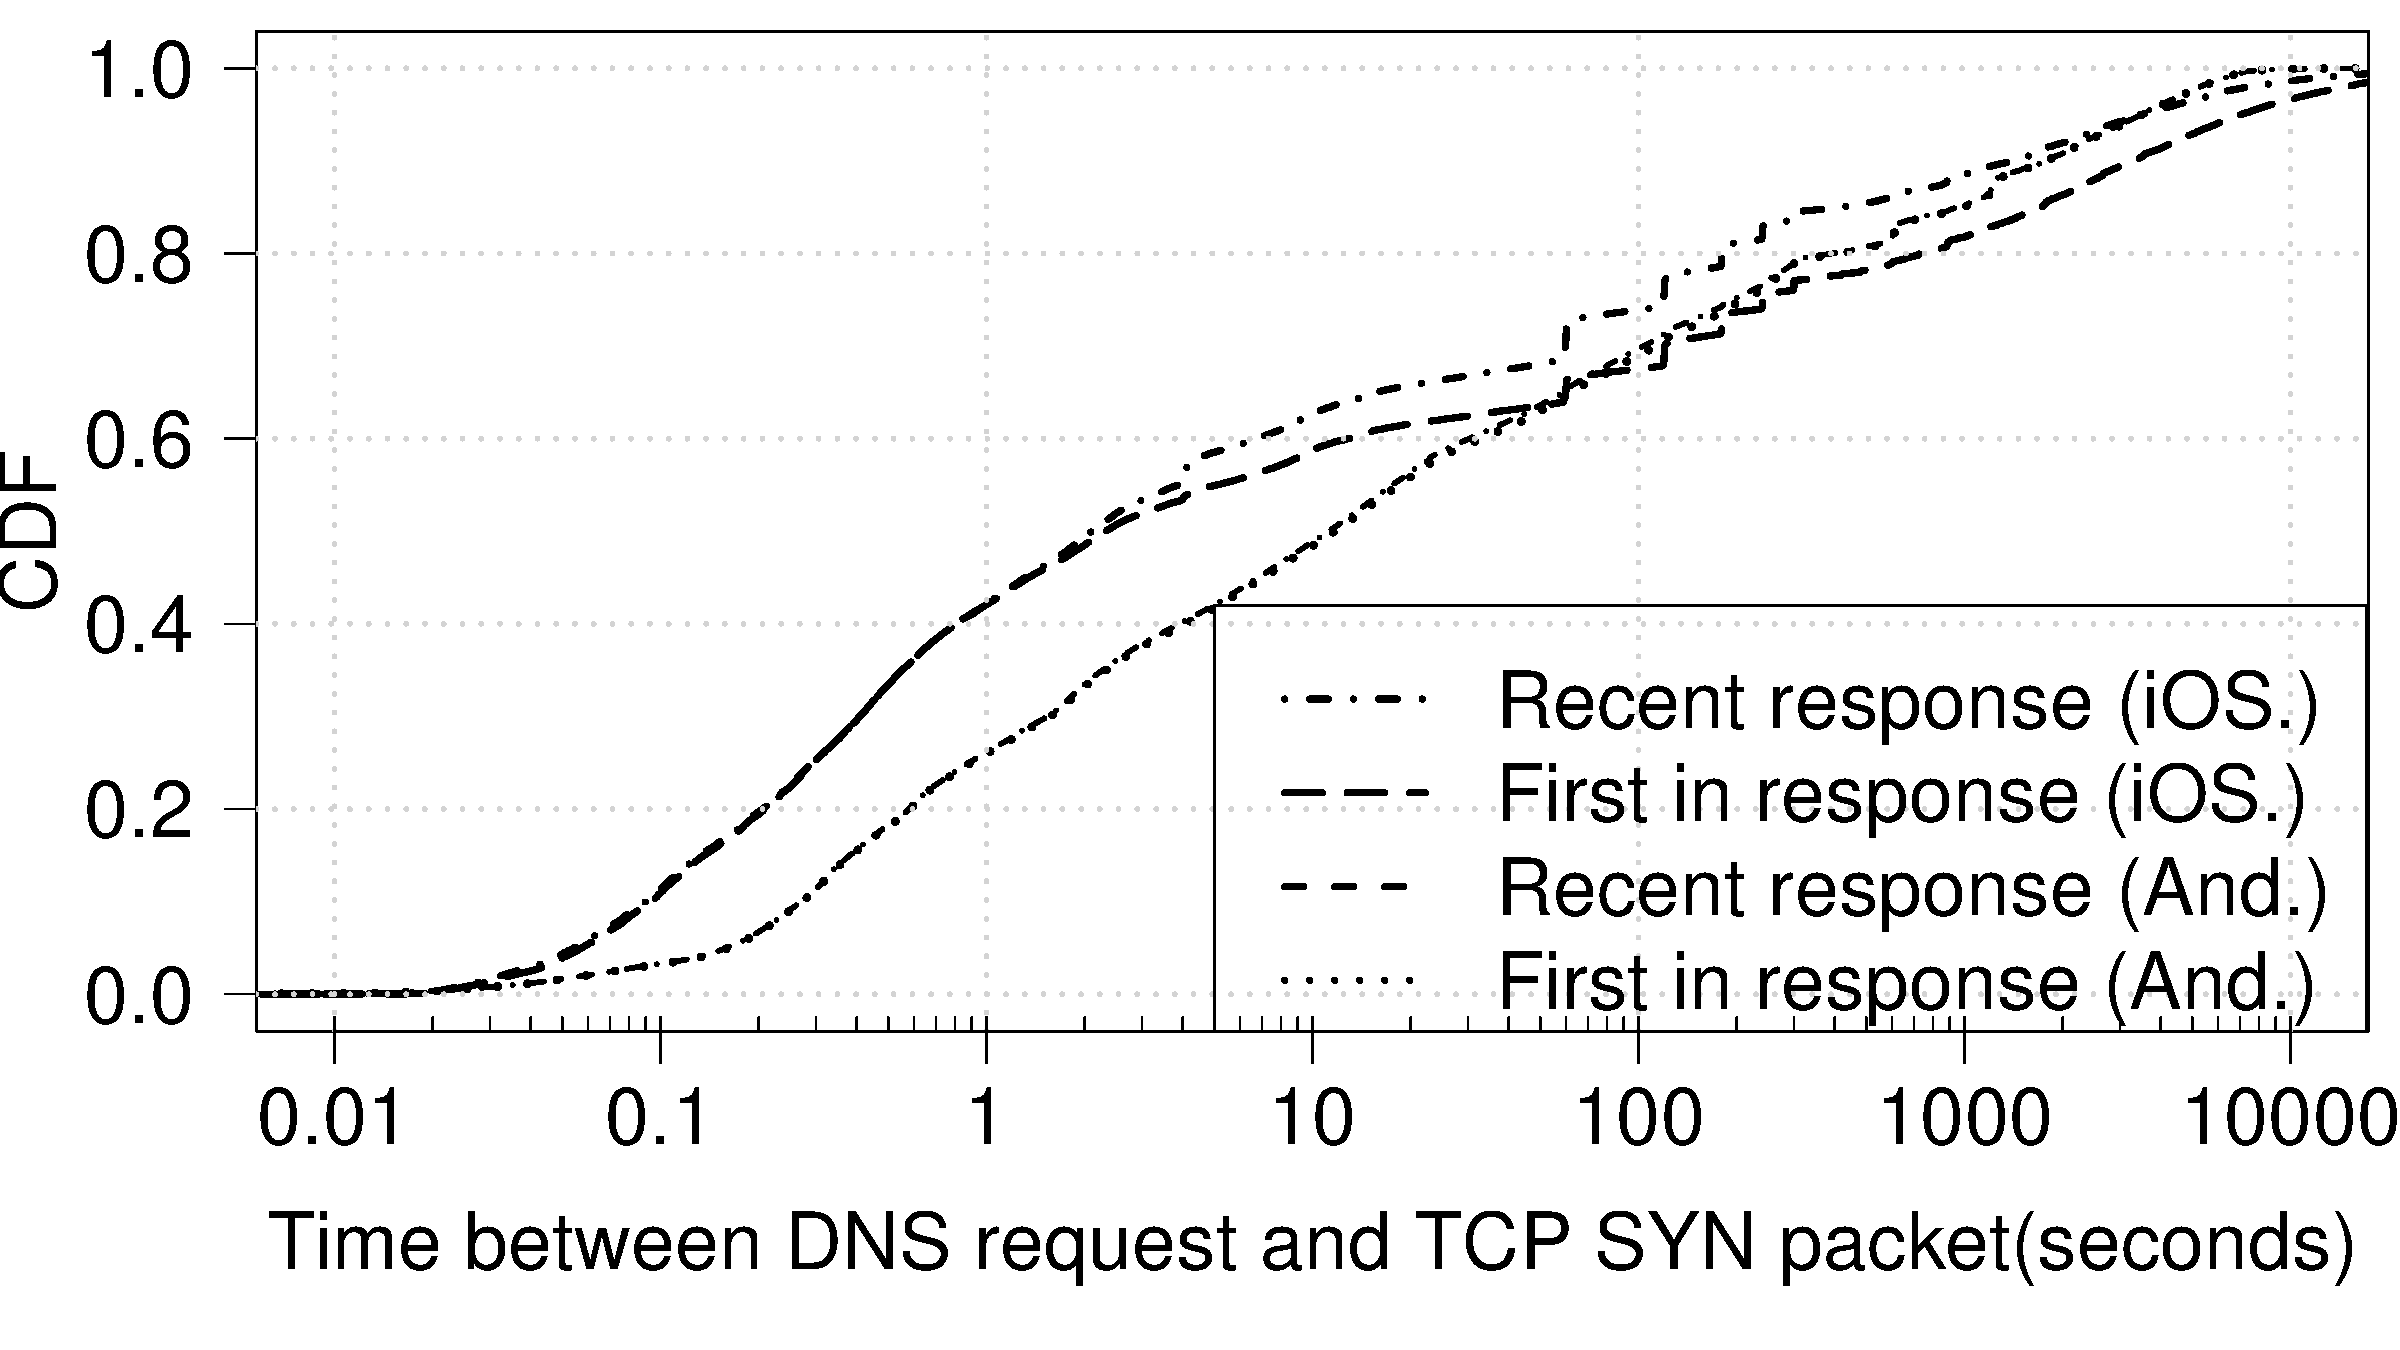
\includegraphics[width=\columnwidth]{plots/sslanalysis_dns_timediff_distrib.pdf}
% \caption{DNS SSL}
% \label{fig:sslclassification-dns-timedistrib}
% \end{figure}
